% !TeX program = xelatex
% !TeX encoding = UTF-8
% !BIB program = biber

%% 广西大学硕博学位论文模板
%% Schrodinger Blume 修改制作，符合 2026 年规范
%% 欢迎闲鱼找「薛定谔之花_」下单
%% 我的邮箱：junhaowu_hit@163.com

%% 主文件仅用于修改信息、配置和添加章节
%% 应尽可能保持简洁
%% 编译应在此文件进行

\documentclass{gxuthesis}
% 若参考文献使用 GB/T 7714—2025 规范：
% \documentclass[gb7714-2025]{gxuthesis}



% —— 文献数据库 ——
\addbibresource{参考文献/ref1.bib}
\addbibresource{参考文献/ref2.bib}



\begin{document}



% 载入「封面、扉页、声明」定义
%% gxufrontmatter.tex — 广西大学硕博学位论文前置部分
%% 封面 + 扉页 + 声明
%% Schrodinger Blume 修改制作，符合 2026 年规范
%% 欢迎闲鱼找「薛定谔之花_」下单
%% 我的邮箱：junhaowu_hit@163.com

% ——— 用户接口 ———
% 标题换行命令
% \coverbreak     — 仅在封面/扉页换行，其余忽略
% \titlebreak     — \coverbreak 的别名，保留以兼容旧用法
% \headerbreak    — 仅在页眉中换行，其余忽略
% \abstractbreak  — 仅在摘要标题中换行，其余忽略
% \\              — 除书脊外均换行（封面/扉页/页眉/摘要 都换行）
\newcommand{\coverbreak}{\\}
\newcommand{\titlebreak}{\coverbreak}
\newcommand{\abstractbreak}{}
\newcommand{\headerbreak}{}
\providecommand{\degree}{博士} % 博士 / 硕士
\providecommand{\cntitle}{研究题目} % 中文标题
\providecommand{\cntitlespine}{\cntitle} % 书脊标题，默认同封面标题
\providecommand{\entitle}{RESEARCH TITLE} % 英文标题
\providecommand{\pubyear}{2026} % 封面年份
\providecommand{\pubmonth}{3} % 封面月份
\providecommand{\major}{} % 专业名称
\providecommand{\research}{} % 研究方向
\providecommand{\category}{} % 分类号
\providecommand{\schoolcode}{} % 学校代码
\providecommand{\level}{} % 密级
\providecommand{\id}{} % 学号
\providecommand{\logpath}{gxulogo} % 广西大学题字图片路径
\providecommand{\defensedate}{} % 论文答辩日期
\providecommand{\degreedate}{} % 学位授予日期
\providecommand{\defensechair}{} % 答辩委员会主席
\providecommand{\infotableskip}{4em}
\providecommand{\thesisauthor}{}
\providecommand{\supervisor}{}
\providecommand{\cosupervisor}{}
\providecommand{\college}{}
% 声明页用户接口
\providecommand{\statementpdf}{gxustatement.pdf}
\providecommand{\statementauthor}{}
\providecommand{\statementauthordate}{}
\providecommand{\statementsupervisor}{}
\providecommand{\statementsupervisordate}{}
\providecommand{\statementphone}{}
\providecommand{\statementemail}{}
% 位置接口
\providecommand{\statementauthorx}{202pt}
\providecommand{\statementauthory}{247.65pt}
\providecommand{\statementauthordatex}{370.5pt}
\providecommand{\statementauthordatey}{247.65pt}
\providecommand{\statementsupervisorx}{202pt}
\providecommand{\statementsupervisory}{222.325pt} % 25.325
\providecommand{\statementsupervisordatex}{370.5pt}
\providecommand{\statementsupervisordatey}{222.325pt}
\providecommand{\statementphonex}{202pt}
\providecommand{\statementphoney}{197pt}
\providecommand{\statementemailx}{398.5pt}
\providecommand{\statementemaily}{197pt}

% 默认不盲审，\gxublindtrue 启用盲审
\newif\ifgxublind
\gxublindfalse

% 默认页眉：横线 + 左侧「广西大学X学位论文」+ 右侧「论文标题」
% 盲审版本（\gxublindtrue）：横线 + 右侧「论文标题」，不显示左侧文字（2026 年新规范）
% 完全隐藏页眉版本：\gxunoheadertrue 启用，横线、左右文字都不显示
\newif\ifgxunoheader
\gxunoheaderfalse

% 书脊默认单列，\gxuspinedoublecoltrue 启用双列
\newif\ifgxuspinedoublecol
\gxuspinedoublecolfalse

% 默认显示书脊，\gxuspinefalse 不显示书脊
\newif\ifgxuspine
\gxuspinetrue

% 书脊单列模式下，默认「字母不旋转」，\gxuspinerotatelettertrue 启用字母旋转
\newif\ifgxuspinerotateletter
\gxuspinerotateletterfalse

% —— 封面 ——
\newcommand{\gxuVertChar}[1]{\hbox{\zihao{3}\bfseries\ifnum\XeTeXcharclass`#1>0\ifnum`#1="2014\leavevmode\unskip\rotatebox{-90}{#1}\else\ifnum`#1="2015\leavevmode\unskip\rotatebox{-90}{#1}\else#1\fi\fi\else\leavevmode\unskip\ifgxuspinerotateletter\rotatebox{-90}{#1}\else\makebox[16pt][c]{#1}\fi\fi}}

\newcommand{\gxuVertCharDouble}[1]{%
  \hbox to \dimexpr16pt\relax{\hss\zihao{3}\bfseries#1\hss}%
} % 书脊两列模式下，两列文字的间距

\newcommand{\gxuVertText}[1]{%
  \begingroup
  \let\\\relax
  \let\titlebreak\relax
  \let\coverbreak\relax
  \let\abstractbreak\relax
  \let\headerbreak\relax
  \newif\ifgxulastdash
  \gxulastdashfalse
  \def\gxuparsevert##1{%
    \ifx##1\gxuend\else
      \ifx##1\relax\else
        \ifnum\XeTeXcharclass`##1>0
          \ifnum`##1="2014
            \ifgxulastdash\vskip-5pt\else\vskip-18.5pt\fi
            \gxulastdashtrue
          \else\ifnum`##1="2015
            \ifgxulastdash\vskip-5pt\else\vskip-18.5pt\fi
            \gxulastdashtrue
          \else
            \gxulastdashfalse
          \fi\fi
        \else
          \ifgxuspinerotateletter\vskip-8pt\fi
          \gxulastdashfalse
        \fi
        \gxuVertChar{##1}%
      \fi
      \expandafter\gxuparsevert
    \fi
  }%
  \vbox{\baselineskip=1\dimexpr21.5pt\relax\expandafter\gxuparsevert#1\gxuend}%
  \endgroup
}

\newcounter{gxuVTDcount}
\newcommand{\gxuVertTextDouble}[1]{%
  \begingroup
  \let\\\relax
  \let\titlebreak\relax
  \let\coverbreak\relax
  \let\abstractbreak\relax
  \let\headerbreak\relax
  \setcounter{gxuVTDcount}{0}%
  \def\gxuVTDfirst{}%
  \def\gxuVTDparse##1{%
    \ifx##1\gxuend\else
      \ifx##1\relax\else
        \ifodd\value{gxuVTDcount}%
          \hbox{\gxuVTDfirst\gxuVertCharDouble{##1}}%
        \else
          \def\gxuVTDfirst{\gxuVertCharDouble{##1}}%
        \fi
        \stepcounter{gxuVTDcount}%
      \fi
      \expandafter\gxuVTDparse
    \fi
  }%
  \vbox{%
    \baselineskip=21.5pt
    \lineskip=0pt
    \lineskiplimit=0pt
    \expandafter\gxuVTDparse#1\gxuend
    \ifodd\value{gxuVTDcount}%
      \hbox{\gxuVTDfirst}%
    \fi
  }%
  \endgroup
}

\def\gxuparsevert#1{%
  \ifx#1\gxuend\else
    \gxuVertChar{#1}%
    \expandafter\gxuparsevert
  \fi
}
\def\gxuend{\gxuend}

\newcommand{\makecoverpageone}{%
\begin{titlepage}
\newgeometry{left=0cm, right=0cm, top=0cm, bottom=0cm}
\begin{tikzpicture}[remember picture, overlay, transform canvas={yshift=-10.5pt}]

    \ifgxuspine
    \node[anchor=west, draw, line width=.75pt,
          minimum height=26.97cm, minimum width=1.67cm] at
        ([shift={(21.25pt, 11.85pt)}]current page.west)
        {};

    \node[anchor=north] at
        ([shift={(45pt, -48.25pt)}]current page.north west)
        {\gxuVertText{\degree}};

    \node[anchor=north] at
        ([shift={(45pt, -108.75pt)}]current page.north west)
        {\gxuVertText{\thesisauthor}};

    \node[anchor=center] at ([shift={(45pt, -28pt)}]current page.west)
        {\ifgxuspinedoublecol\gxuVertTextDouble{\cntitle}\else\gxuVertText{\cntitle}\fi};

    \node[anchor=center, rotate=-90] at
        ([shift={(45pt, 76.25pt)}]current page.south west)
        {\zihao{3}\bfseries\pubyear};
    \fi

    \node[anchor=north east, draw, line width=1.5pt,
      inner xsep=14.75pt, inner ysep=7.5pt, align=center] at
    ([shift={(-65.75pt, -176pt)}]current page.north east)
    {\lishu\zihao{3}
     \ifgxulishufound
         \CJKfontspec{simli.ttf}[Path=字体/, RawFeature={embolden=2.5}]%
     \fi
     \degree \\[1.5pt]
     \lishu\zihao{3}
     \ifgxulishufound
         \CJKfontspec{simli.ttf}[Path=字体/, RawFeature={embolden=2.5}]%
     \fi
     \ifgxuprofessional 专业\fi 学位论文};

    % 标题行距：\fontsize 必须放在 \node 之外
    % 因为 TikZ 内部 \parbox/minipage 启动时
    % \@parboxrestore 会把 \baselineskip 重置为外层 \normalbaselineskip
    % 若写在节点内，paragraph builder 实际收到的是外层 strut
    % 导致自动换行与 \\、\titlebreak 视觉不一致
    {\fontsize{26bp}{33bp}\selectfont
    \node[anchor=north, text width=17cm, align=flush center] at
        ([shift={(5pt, 141.8pt)}]current page.center)
        {\textbf{\cntitle}};}

    \node[anchor=center] at
        ([shift={(5pt, -95.5pt)}]current page.center)
        {\zihao{1}\textbf{\thesisauthor}};

    \ifgxublind\else
    \node[anchor=south, opacity=1] at
        ([shift={(5pt, -270.25pt)}]current page.center)
        {
\includegraphics[width=5.7cm]{gxulogo.png}};
    \fi

    \node[anchor=center] at
        ([shift={(5pt, -287pt)}]current page.center)
        {\zihao{-2}
         \textbf{\zhdigits{\pubyear} 年\hspace{.5em}\zhnumber{\pubmonth}\hspace{.5em}月}};

\end{tikzpicture}%
\restoregeometry
\end{titlepage}
}



% —— 扉页 ——
\newcommand{\makecoverpagetwo}{%
\begin{titlepage}

\vspace*{-14.5pt}

\ifgxublind
    \vspace*{2.75pt}
\else
    \vspace*{-20pt}
    \begin{tikzpicture}[remember picture, overlay]
        \node[anchor=center, opacity=1] at ([shift={(-2pt, 224.25pt)}]current page.center) {%
            
\includegraphics[width=6.28cm]{gxulogo.png}%
        };
    \end{tikzpicture}
\fi

% 分类号 / 学校代码 / 密级
\noindent
\begin{tabular}{@{}l@{}l@{\hspace{45.5pt}}l@{}l@{}}
    \ifdefempty{\category}{}{\zihao{-3}分类号&
    \uline{\makebox[11.5em][c]{\zihao{-3}\category}}}%
    \ifdefempty{\schoolcode}{}{&
    \zihao{-3}学校代码&
    \uline{\makebox[10em][c]{\zihao{-3}\schoolcode}}}
\end{tabular}

\vspace{12pt}

\noindent
\begin{tabular}{@{}l@{}l@{\hspace{45.5pt}}l@{}l@{}}
    \ifdefempty{\level}{}{\zihao{-3}密级&
    \uline{\makebox[12.75em][c]{\zihao{-3}\level}}}%
    \ifdefempty{\id}{}{&
    \zihao{-3}学号&
    \uline{\makebox[12.5em][c]{\zihao{-3}\id}}}
\end{tabular}

\vspace{88.25pt}

% 论文类型
\begin{center}
    {\lishu\zihao{2}
     \ifgxulishufound
         \CJKfontspec{simli.ttf}[Path=字体/, RawFeature={embolden=2.5}]%
     \fi
     \degree \ifgxuprofessional 专业\fi 学位论文}
\end{center}

\vspace{-2pt}

% 中文标题
\begin{center}
    \begin{minipage}{\textwidth}
        \centering
        \zihao{-1}\bfseries
        \setlength{\baselineskip}{38.5bp}%
        \cntitle
    \end{minipage}
\end{center}

\vspace{6.5pt}

% 英文标题
\begin{center}
    \begin{minipage}{\textwidth}
        \centering
        \zihao{2}
        \setlength{\baselineskip}{31.75bp}%
        \entitle
    \end{minipage}
\end{center}

\vspace{\infotableskip}

% 判断底部三个字段是否有任意一个非空
\newif\ifgxushowbottom
\gxushowbottomfalse
\ifdefempty{\defensedate}{}{\gxushowbottomtrue}
\ifdefempty{\degreedate}{}{\gxushowbottomtrue}
\ifdefempty{\defensechair}{}{\gxushowbottomtrue}

% 上方信息表格，随文字流动（怕有人标题太长了）
\begin{center}
\begin{tabular}{@{}r@{\hspace{1em}}l@{}}
    \ifdefempty{\thesisauthor}{}{%
    \zihao{-3}\bfseries 作者姓名：&
    \zihao{-3}\underline{\makebox[11em][c]{\thesisauthor}} \\[10.2pt]}
    \ifdefempty{\supervisor}{}{%
    \zihao{-3}\bfseries 指导教师：&
    \zihao{-3}\underline{\makebox[11em][c]{\supervisor}} \\[10.2pt]}
    \ifdefempty{\cosupervisor}{}{%
    \zihao{-3}\bfseries 合作导师：&
    \zihao{-3}\underline{\makebox[11em][c]{\cosupervisor}} \\[10.2pt]}
    \ifdefempty{\major}{}{%
    \zihao{-3}\bfseries 专业名称：&
    \zihao{-3}\underline{\makebox[11em][c]{\major}} \\[10.2pt]}
    \ifdefempty{\research}{}{%
    \zihao{-3}\bfseries 研究方向：&
    \zihao{-3}\underline{\makebox[11em][c]{\research}} \\[10.2pt]}
    \ifdefempty{\college}{}{%
    \zihao{-3}\bfseries 所在学院：&
    \zihao{-3}\underline{\makebox[11em][c]{\college}} \\[10.2pt]}
\end{tabular}
\end{center}

% 底部答辩信息，固定位置
\begin{tikzpicture}[remember picture, overlay]
    \ifgxushowbottom
    \node[anchor=west] at ([shift={(-223.25pt, -289pt)}]current page.center) {%
        \begin{tabular}{@{}l@{}l@{}l@{}l@{}}
            \ifdefempty{\defensedate}{&}{%
            \zihao{-3}\bfseries 论文答辩日期\hspace*{.6em}&
            \zihao{-3}\simsun\underline{\makebox[8.7em][l]{\CJKsetecglue{\hspace{.25em}}\defensedate}}}%
            \ifdefempty{\degreedate}{&}{%
            &\zihao{-3}\bfseries 学位授予日期\hspace*{.6em}&
            \zihao{-3}\simsun\underline{\makebox[8.2em][l]{\CJKsetecglue{\hspace{.25em}}\degreedate}}} \\
        \end{tabular}
    };
    \node[anchor=west] at ([shift={(-223.25pt, -322.75pt)}]current page.center) {%
        \begin{tabular}{@{}l@{}l@{}}
            \ifdefempty{\defensechair}{}{%
            \zihao{-3}\bfseries 答辩委员会主席\hspace*{.5em}&
            \zihao{-3}\underline{\makebox[\maxof{6.5em}{\widthof{\zihao{-3}\defensechair}+0em}][l]{\defensechair}}} \\
        \end{tabular}
    };
    \fi
\end{tikzpicture}

\restoregeometry
\end{titlepage}
}



% —— 声明 ——
\providecommand{\secretperiod}{}

\newcommand{\secretperiodnodes}{%
    \ifdefempty{\secretperiod}{%
        \node at (1.1,-15.15) {\zihao{-4}√};%
    }{%
        \node at (1.1,-14.25) {\zihao{-4}√};%
        \node at (3.96,-14.2425) {\zihao{4}\secretperiod};%
    }%
}%

\newcommand{\makestatementoverlay}{%
    \thispagestyle{empty}%
    \begin{tikzpicture}[remember picture, overlay]
        \secretperiodnodes
        \node[anchor=west] at ([shift={(\statementauthorx, \statementauthory)}]current page.south west)
            {\zihao{4}\statementauthor};
        \node[anchor=west] at ([shift={(\statementauthordatex, \statementauthordatey)}]current page.south west)
            {\zihao{4}\statementauthordate};
        \node[anchor=west] at ([shift={(\statementsupervisorx, \statementsupervisory)}]current page.south west)
            {\zihao{4}\statementsupervisor};
        \node[anchor=west] at ([shift={(\statementsupervisordatex, \statementsupervisordatey)}]current page.south west)
            {\zihao{4}\statementsupervisordate};
        \node[anchor=west] at ([shift={(\statementphonex, \statementphoney)}]current page.south west)
            {\zihao{4}\statementphone};
        \node[anchor=west] at ([shift={(\statementemailx, \statementemaily)}]current page.south west)
            {\zihao{4}\statementemail};
    \end{tikzpicture}%
}

\newcommand{\makestatement}{%
    \includepdf[pages={1},
        pagecommand={\makestatementoverlay}%
    ]{\statementpdf}%
}



% —— 调用命令 ——
\newcommand{\makecover}{%
    \makecoverpageone
    \makecoverpagetwo
}

% 默认生成声明页，改为 \gxustatementfalse 则不生成
\newif\ifgxustatement
\gxustatementtrue

% 默认学术学位，\gxuprofessionaltrue 启用专业学位
\newif\ifgxuprofessional
\gxuprofessionalfalse



% —— 配置基本信息 ——
\renewcommand{\degree}{硕士} % 博士 / 硕士
% \gxuprofessionaltrue % 默认「学术学位」，取消注释则切换到「专业学位」
% ————————————————————————————————————————————
% 如果「盲审」，则「启用」下面这行命令
% 将不显示「广西大学图标」与「页眉」
% \gxublindtrue
% ————————————————————————————————————————————
% 「留空/注释掉」则对应栏目完全「不显示」
% 如果用「空格占位」则可以只显示「左侧文字」和「下划线」
\renewcommand{\category}{（中图分类号）} % 分类号
\renewcommand{\schoolcode}{} % 学校代码
\renewcommand{\level}{   } % 密级
% \renewcommand{\id}{2211399999} % 学号
% ————————————————————————————————————————————
% 「留空/注释掉」则对应栏目完全「不显示」
% 如果用「空格占位」则可以只显示「左侧文字」和「下划线」
\renewcommand{\thesisauthor}{张三} % 作者姓名
\renewcommand{\supervisor}{李四} % 指导教师
\renewcommand{\cosupervisor}{王五} % 合作导师
\renewcommand{\major}{物理学} % 专业名称
\renewcommand{\research}{量子通信} % 研究方向
\renewcommand{\college}{物理科学与工程技术学院} % 所在学院
% ————————————————————————————————————————————
% 「留空/注释掉」则对应栏目完全「不显示」
% 如果用「空格占位」则可以只显示「左侧文字」和「下划线」
\renewcommand{\defensedate}{2025年6月1日} % 论文答辩日期
\renewcommand{\degreedate}{2025年6月30日} % 学位授予日期
\renewcommand{\defensechair}{   } % 答辩委员会主席
% ————————————————————————————————————————————
% 标题「换行」机制见模板给的示例（节 2.2）
\renewcommand{\cntitle}{沙基太阳能界面蒸发器的构建及其\\ 光热蒸汽转换性能研究} % 中文标题
% 如果中文标题中有「字母」的话，「书脊」的表现「可能不好」
% \gxuspinedoublecoltrue % 书脊默认按「单列」排版，取消注释则按「双列」排版
% \gxuspinefalse % 默认显示书脊，取消注释则不显示书脊

\renewcommand{\entitle}{Research Title} % 英文标题，换行只能用 \\
% ————————————————————————————————————————————
% 年份和数字都要写阿拉伯数字
\renewcommand{\pubyear}{2026} % 封面年份
\renewcommand{\pubmonth}{6} % 封面月份
% ————————————————————————————————————————————
% 扉页中，「英文标题」与「信息表格」的间隙，默认 4em，按需修改
% \renewcommand{\infotableskip}{4em}



% —— 配置声明页信息 ——
% \gxustatementfalse % 默认生成声明页，取消此行注释则不生成声明页
% ————————————————————————————————————————————
% 不保密（默认）：「不写」或「留空」
% \renewcommand{\secretperiod}{}
% 若保密则填写期限：
\renewcommand{\secretperiod}{三}
% ————————————————————————————————————————————
\renewcommand{\statementauthor}{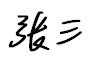
\includegraphics[height=2em]{签名/作者签名.png}}
\renewcommand{\statementauthordate}{2026.06.01}
% ————————————————————————————————————————————
\renewcommand{\statementsupervisor}{
\includegraphics[height=2em]{签名/导师签名.png}}
\renewcommand{\statementsupervisordate}{2026.06.02}
% ————————————————————————————————————————————
\renewcommand{\statementphone}{13812345678}
\renewcommand{\statementemail}{xxx@st.gxu.edu.cn}



% —— 前置部分（封面 / 摘要 / 目录）——
\makefrontmatter
    {\cntitle}
    {\entitle}
    {论文内容/中文摘要}
    {论文内容/英文摘要}
% ————————————————————————————————————————————
% — 辅助目录 — 不需要则注释/删掉相应命令
\gxulistoffigures % 插图清单
% ————————————————————————————————————————————
% 附表清单
\clearpage\gxulistoftables
% ————————————————————————————————————————————
% 缩略语清单
\clearpage\gxulistofabbr
\begin{longtable}{@{}lll@{}}
    \textbf{\heiti 缩略语} & \textbf{\heiti 英文全称} & \textbf{\heiti 中文全称} \\
    \endfirsthead
    \textbf{\heiti 缩略语} & \textbf{\heiti 英文全称} & \textbf{\heiti 中文全称} \\
    \endhead
    AI    & Artificial Intelligence                        & 人工智能 \\
    ANN   & Artificial Neural Network                      & 人工神经网络 \\
    API   & Application Programming Interface              & 应用程序接口 \\
    AR    & Augmented Reality                              & 增强现实 \\
    BERT  & Bidirectional Encoder Representations from Transformers & 双向编码器表示 \\
    BIM   & Building Information Modeling                  & 建筑信息模型 \\
    CAD   & Computer-Aided Design                          & 计算机辅助设计 \\
    CAM   & Computer-Aided Manufacturing                   & 计算机辅助制造 \\
    CEO   & Chief Executive Officer                        & 首席执行官 \\
    CFO   & Chief Financial Officer                        & 首席财务官 \\
    CIO   & Chief Information Officer                      & 首席信息官 \\
    CRM   & Customer Relationship Management               & 客户关系管理 \\
    CNN   & Convolutional Neural Network                   & 卷积神经网络 \\
    CPU   & Central Processing Unit                        & 中央处理器 \\
    CSR   & Corporate Social Responsibility                & 企业社会责任 \\
    CTO   & Chief Technology Officer                       & 首席技术官 \\
    DL    & Deep Learning                                  & 深度学习 \\
    DNA   & Deoxyribonucleic Acid                          & 脱氧核糖核酸 \\
    ERP   & Enterprise Resource Planning                   & 企业资源规划 \\
    ESG   & Environmental, Social and Governance           & 环境、社会与治理 \\
    FDI   & Foreign Direct Investment                      & 外商直接投资 \\
    GDP   & Gross Domestic Product                         & 国内生产总值 \\
    GIS   & Geographic Information System                  & 地理信息系统 \\
    GMM   & Generalized Method of Moments                  & 广义矩估计法 \\
    GNP   & Gross National Product                         & 国民生产总值 \\
    GPU   & Graphics Processing Unit                       & 图形处理器 \\
    GRU   & Gated Recurrent Unit                           & 门控循环单元 \\
    GXU   & Guangxi University                             & 广西大学 \\
    HR    & Human Resources                                & 人力资源 \\
    HTML  & HyperText Markup Language                      & 超文本标记语言 \\
    HTTP  & HyperText Transfer Protocol                    & 超文本传输协议 \\
    IIoT  & Industrial Internet of Things                  & 工业物联网 \\
    IoT   & Internet of Things                             & 物联网 \\
    IP    & Intellectual Property                          & 知识产权 \\
    IPO   & Initial Public Offering                        & 首次公开募股 \\
    IT    & Information Technology                         & 信息技术 \\
    KPI   & Key Performance Indicator                      & 关键绩效指标 \\
    LSTM  & Long Short-Term Memory                         & 长短期记忆网络 \\
    M\&A  & Mergers and Acquisitions                       & 兼并与收购 \\
    ML    & Machine Learning                               & 机器学习 \\
    MLP   & Multilayer Perceptron                          & 多层感知机 \\
    NLP   & Natural Language Processing                    & 自然语言处理 \\
    OLS   & Ordinary Least Squares                         & 普通最小二乘法 \\
    P2P   & Peer to Peer                                   & 点对点 \\
    PDF   & Probability Density Function                   & 概率密度函数 \\
    PLC   & Programmable Logic Controller                  & 可编程逻辑控制器 \\
    PPP   & Public-Private Partnership                     & 公私合营 \\
    QKD   & Quantum Key Distribution                       & 量子密钥分发 \\
    R\&D  & Research and Development                       & 研究与开发 \\
    RFID  & Radio Frequency Identification                 & 射频识别 \\
    RNN   & Recurrent Neural Network                       & 循环神经网络 \\
    ROA   & Return on Assets                               & 资产收益率 \\
    ROE   & Return on Equity                               & 净资产收益率 \\
    ROI   & Return on Investment                           & 投资回报率 \\
    SCM   & Supply Chain Management                        & 供应链管理 \\
    SME   & Small and Medium-sized Enterprise              & 中小型企业 \\
    SQL   & Structured Query Language                      & 结构化查询语言 \\
    SVM   & Support Vector Machine                         & 支持向量机 \\
    TFP   & Total Factor Productivity                      & 全要素生产率 \\
    UI    & User Interface                                 & 用户界面 \\
    URL   & Uniform Resource Locator                       & 统一资源定位符 \\
    VAR   & Vector Autoregression                          & 向量自回归 \\
    VR    & Virtual Reality                                & 虚拟现实 \\
\end{longtable}
% ————————————————————————————————————————————
% 符号清单
\clearpage\gxulistofsymbols
\begin{longtable}{@{}lll@{}}
    \textbf{\heiti 符号} & \textbf{\heiti 含义} & \textbf{\heiti 单位} \\
    \endfirsthead
    \textbf{\heiti 符号} & \textbf{\heiti 含义} & \textbf{\heiti 单位} \\
    \endhead
    $a$             & 尺度因子                  & — \\
    $A$             & 面积                      & m\textsuperscript{2} \\
    $\alpha$        & 热扩散系数                & m\textsuperscript{2}/s \\
    $\beta$         & 热膨胀系数                & K\textsuperscript{-1} \\
    $c$             & 光速                      & m/s \\
    $c_p$           & 定压比热容                & J/(kg·K) \\
    $C$             & 电容                      & F \\
    $\chi$          & 磁化率                    & — \\
    $d$             & 特征长度                  & m \\
    $D$             & 扩散系数                  & m\textsuperscript{2}/s \\
    $\delta$        & 边界层厚度                & m \\
    $e$             & 基本电荷                  & C \\
    $E$             & 电场强度                  & V/m \\
    $\varepsilon$   & 应变张量                  & — \\
    $\eta$          & 动力黏度                  & Pa·s \\
    $f$             & 频率                      & Hz \\
    $F$             & 力                        & N \\
    $g$             & 重力加速度                & m/s\textsuperscript{2} \\
    $G$             & 剪切模量                  & Pa \\
    $\gamma$        & 比热比                    & — \\
    $h$             & 普朗克常数                & J·s \\
    $H$             & 磁场强度                  & A/m \\
    $\hbar$         & 约化普朗克常数            & J·s \\
    $I$             & 电流                      & A \\
    $j$             & 电流密度                  & A/m\textsuperscript{2} \\
    $k$             & 波尔兹曼常数              & J/K \\
    $k_t$           & 导热系数                  & W/(m·K) \\
    $\kappa$        & 曲率                      & m\textsuperscript{-1} \\
    $\lambda$       & 波长                      & m \\
    $\Lambda$       & 平均自由程                & m \\
    $L$             & 特征长度                  & m \\
    $m$             & 质量                      & kg \\
    $M$             & 摩尔质量                  & kg/mol \\
    $\mu$           & 化学势                    & J/mol \\
    $\mu_0$         & 真空磁导率                & H/m \\
    $n$             & 粒子数密度                & m\textsuperscript{-3} \\
    $N$             & 总粒子数                  & — \\
    $\nu$           & 运动黏度                  & m\textsuperscript{2}/s \\
    $\omega$        & 角频率                    & rad/s \\
    $\Omega$        & 立体角                    & sr \\
    $p$             & 压强                      & Pa \\
    $P$             & 功率                      & W \\
    $\phi$          & 电势                      & V \\
    $\Phi$          & 磁通量                    & Wb \\
    $\psi$          & 波函数                    & — \\
    $q$             & 热流密度                  & W/m\textsuperscript{2} \\
    $Q$             & 热量                      & J \\
    $r$             & 径向坐标                  & m \\
    $R$             & 气体常数                  & J/(mol·K) \\
    $\rho$          & 密度                      & kg/m\textsuperscript{3} \\
    $s$             & 比熵                      & J/(kg·K) \\
    $S$             & 熵                        & J/K \\
    $\sigma$        & 应力张量                  & Pa \\
    $\sigma_0$      & 斯特藩-玻尔兹曼常数       & W/(m\textsuperscript{2}·K\textsuperscript{4}) \\
    $t$             & 时间                      & s \\
    $T$             & 温度                      & K \\
    $\tau$          & 剪切应力                  & Pa \\
    $u$             & 速度分量（$x$方向）       & m/s \\
    $U$             & 内能                      & J \\
    $v$             & 速度分量（$y$方向）       & m/s \\
    $V$             & 体积                      & m\textsuperscript{3} \\
    $w$             & 速度分量（$z$方向）       & m/s \\
    $W$             & 功                        & J \\
\end{longtable}
% ————————————————————————————————————————————
% 术语表
\clearpage\gxulistofterms
\begin{longtable}{@{}p{9em}p{10em}p{\dimexpr\textwidth-9em-10em}@{}}
    \textbf{\heiti 术语} & \textbf{\heiti 英文} & \textbf{\heiti 释义} \\
    \endfirsthead
    \textbf{\heiti 术语} & \textbf{\heiti 英文} & \textbf{\heiti 释义} \\
    \endhead
    暗能量 & Dark Energy   & 导致宇宙加速膨胀的未知能量形式 \\
    暗物质 & Dark Matter   & 不与电磁力产生作用的假想物质 \\
    波函数 & Wave Function & 描述量子系统状态的复值函数 \\
\end{longtable}



% —— 正文 ——
\startmainmatter % 加载正文配置
% \gxustretchwide % 行间距切换到 25 磅
% \gxuafternamenarrrow % 标题文字与编号间距设置为半个汉字宽
\section{模板使用说明}

本模板依据广西大学学位论文格式规范，基于 \TeX{} Live 2025 制作（最低测试至 \TeX{} Live 2023），默认行距对应 Word 中的 1.25 倍行距效果\footnote{"文档网格——只指定行网格——每页 44 行"下的表现。}。如需切换至 25 磅行距，可在正文开始前调用 \verb|\gxustretchwide| 命令；如需切换回默认行距，调用 \verb|\gxustretchnormal|。需要注意的是，25 磅行距仅调整正文文字的行距，其余格式参数未做相应匹配，实际效果可能欠佳，不建议使用。

\subsection{声明}

本模板作者并非广西大学在读或毕业学生，与广西大学不存在任何隶属关系。本模板参考了学校内流传的不知名 \LaTeX{} 模板，并在此基础上进行了大量修改与重构；若原作者认为本模板侵犯了其权益，请联系作者，将立即删除相关内容。

模板中使用的广西大学题字图片提取自广西大学官方发布的 Word 学位论文模板，仅供本模板排版使用，\textbf{严禁用于其他任何用途}。作者无意侵犯广西大学的任何权益，若校方认为此使用方式不当，请联系作者处理。

由于作者与广西大学并无关联，无法持续获取最新格式规范，\textbf{本模板在发布后将不再主动维护}。若广西大学日后更新学位论文格式要求，本模板可能无法及时跟进。欢迎有意愿的同学或开发者在本模板基础上继续维护与更新，\textbf{更新时请在显著位置保留对原作者的署名：薛定谔之花/Schrodinger Blume}。

\subsection{字体}

本模板使用中易系列字体排版，包括中易宋体、中易黑体与中易隶书。请注意，上述字体均为微软公司的商业字体，受版权保护，\textbf{请勿将字体文件用于商业用途，亦请勿将其上传至公开网络}。

若您的操作系统为 Windows，上述字体通常已随系统预装，模板将自动识别并加载，无需额外操作。

若您的操作系统为 macOS 或 Linux，则需自行获取字体并安装。若您使用在线编译平台（如 Overleaf、TeXPage\footnote{TeXPage 平台支持中易宋体及中易黑体，仅需上传中易隶书字体文件。}等），则应将字体文件放置于项目根目录下的 \texttt{字体/} 文件夹中。文件命名规则如下：
\begin{itemize}
    \item 中易宋体：\texttt{simsun.ttc}（优先）或 \texttt{simsun.ttf}
    \item 中易黑体：\texttt{simhei.ttf}
    \item 中易隶书：\texttt{simli.ttf}
\end{itemize}

注意文件名及扩展名须\textbf{全部小写}，否则将无法被正确识别。若上述字体均无法获取，模板将自动回退至系统默认字体，仍可正常编译，但排版效果或与预期有所差异\footnote{宋体和黑体理论上将退回至 Fandol 系列字体，隶书将用加粗黑体代替。}。

\subsection{标题的使用}

本模板支持四级正式编号标题（\verb|\section| 至 \verb|\paragraph|），标题文字与编号之间的间距默认为一个汉字宽度（\verb|1em|）。如需调整为半个汉字宽度，可在正文开始前调用 \verb|\gxuafternamenarrrow| 命令。

\subsubsection{五级及以上标题的处理}

根据广西大学模板要求，四级标题（\verb|\paragraph|）之后，应使用数字加圆括号或字母标注五级及以上层次。本模板为此预定义了以下有序列表样式，可通过 \verb|\begin{enumerate}[样式名]| 调用：

\begin{itemize}
    \item \verb|[kuohao]|（括号）：用于第五级，编号格式为（1）（2）（3）……
    \item \verb|[daxie]|（大写字母）：用于第六级，编号格式为 A、B、C……
    \item \verb|[xiaoxie]|（小写字母）：用于第七级，编号格式为 a、b、c……
    \item \verb|[shuzi]|（数字带句点）：备用数字样式，与默认样式的区别在于换行后不缩进
\end{itemize}

以下展示各样式的实际效果：

\paragraph{四级标题}

五级标题使用 \verb|[kuohao]| 样式：
\begin{enumerate}[kuohao]
    \item 五级标题示例
    \item 五级标题示例
\end{enumerate}

六级标题使用 \verb|[daxie]| 样式：
\begin{enumerate}[daxie]
    \item 六级标题示例
    \item 六级标题示例
\end{enumerate}

七级标题使用 \verb|[xiaoxie]| 样式：
\begin{enumerate}[xiaoxie]
    \item 七级标题示例
    \item 七级标题示例
\end{enumerate}

\verb|[shuzi]| 样式与默认数字样式的换行缩进对比：
\begin{enumerate}[shuzi]
    \item 数字样式（无缩进）：数字数字数字数字数字数字数字数字数字数字数字数字数字数字数字数字数字数字数字数字数字数字数字数字数字
    \item 数字样式（无缩进）：数字数字数字数字数字数字数字数字数字数字数字数字数字数字数字数字数字数字数字数字数字数字数字数字数字
\end{enumerate}
\begin{enumerate}
    \item 默认样式（有缩进）：数字数字数字数字数字数字数字数字数字数字数字数字数字数字数字数字数字数字数字数字数字数字数字数字数字
    \item 默认样式（有缩进）：数字数字数字数字数字数字数字数字数字数字数字数字数字数字数字数字数字数字数字数字数字数字数字数字数字
\end{enumerate}
\clearpage
\section{关键注意事项}

\subsection{章节换页}

每一章正文结束后，建议在 \verb|\section| 之前使用 \verb|\clearpage| 命令强制换页，以确保图表等浮动体不会跨章出现。

\subsection{标题换行命令}

本模板定义了专用的标题换行命令 \verb|\titlebreak|\index{huanhangxingwei@换行行为}，用于在不同排版场景下独立控制标题的换行行为。\verb|\titlebreak| 与 \verb|\\| 的区别如表~\ref{tab:titlebreak} 所示。

\begin{table}[H]
    \centering
    \bicaption{标题换行命令在各场景下的行为}{Behavior of title line-break commands in different contexts}
    \label{tab:titlebreak}
    \begin{tabular}{@{}llll@{}}
        \toprule
        命令 & 封面标题 & 书脊标题 & 页眉右侧 \\ \midrule
        \verb|\titlebreak| & 换行 & 忽略 & 忽略 \\
        \verb|\\|           & 换行 & 忽略 & 换行 \\ \bottomrule
    \end{tabular}
\end{table}

使用时需注意以下两点：其一，页眉文字不得超过两行，本模板未对三行及以上页眉做适配，超出时排版效果将与 Word 不一致；其二，当标题在封面页因过长而发生自动换行时，自动换行产生的行间距偏窄（刻意为之），必须在适当位置手动添加换行符并指定行距。具体使用案例参见表~\ref{tab:titlebreak-examples}。

\begin{table}[H]
    \centering
    \bicaption{标题换行命令使用案例}{Usage examples of title line-break commands}
    \label{tab:titlebreak-examples}
    \zihao{-6}
    \begin{tabular}{@{}p{3cm}p{2.75cm}p{5cm}p{5cm}@{}}
        \toprule
        命令写法 & 封面标题 & 书脊（始终不换行） & 页眉 \\ \midrule
        \verb|\renewcommand{\cntitle}{...|\newline\verb|\titlebreak...}| &
        \parbox[t]{5cm}{大型企业与地区社会变迁研究\\——以广西为例} &
        大型企业与地区社会变迁研究——以广西为例 &
        大型企业与地区社会变迁研究——以广西为例 \\[2em]
        \verb|\renewcommand{\cntitle}{...|\newline\verb|\\...}| &
        \parbox[t]{5cm}{大型企业与地区社会变迁研究\\——以广西为例} &
        大型企业与地区社会变迁研究——以广西为例 &
        \parbox[t]{5cm}{大型企业与地区社会变迁研究\\——以广西为例} \\[2em]
        \verb|\renewcommand{\cntitle}{...|\newline\verb|\titlebreak...\\...}| &
        \parbox[t]{5cm}{大型企业\\与地区社会变迁研究\\——以广西为例} &
        大型企业与地区社会变迁研究——以广西为例 &
        \parbox[t]{5cm}{大型企业与地区社会变迁研究\\——以广西为例} \\
        \bottomrule
    \end{tabular}
\end{table}
\clearpage
\section{数学符号与公式规范}\label{equation}

本模板基于 \verb|unicode-math| 宏包处理数学排版，与传统 \verb|amsmath| 在个别命令上存在差异，但已做兼容性处理，绝大多数情况下可直接使用原有命令。

根据 GB/T 3102.11—1993《物理科学和技术中使用的数学符号》，公式中物理量的变量符号用斜体，常量符号用正体。具体规范如下：

\begin{enumerate}[kuohao]
  \item 正文中的数学内容使用 \verb|$…$| 包围，例如 \verb|$A_{italic}$|、\verb|$B_\text{upright}$|、\verb|$C^{中文也支持}$| 编译得到 $A_{italic}$、$B_\text{upright}$、$C^{中文也支持}$\footnote{本模板支持在数学上下标中直接输入中文，无需 \textbackslash text 命令。}。
  \item 数学常数和特殊函数名使用正体，可通过 \verb|\symup{}| 命令实现。本模板预定义了 \verb|\ee|、\verb|\ii|、\verb|\jj|，分别输出自然底数 $\ee$、虚数单位 $\ii$ 和 $\jj$。小写希腊字母的正体形式通过加 \verb|up| 前缀实现，如 $\uppi = 3.14\dots$。
  \item 希腊字母：大写字母默认为正体，斜体形式通过加 \verb|var| 前缀实现，例如 \verb|$\Gamma$| 得到 $\Gamma$，\verb|$\varGamma$| 得到 $\varGamma$；小写字母默认为斜体，正体形式通过加 \verb|up| 前缀实现，例如 \verb|$\gamma$| 得到 $\gamma$，\verb|$\upgamma$| 得到 $\upgamma$。
  \item 微分符号与偏微分符号使用正体，分别用 \verb|\dif| 和 \verb|\partial| 输出 $\dif$ 和 $\partial$。有限增量符号应使用 \verb|\increment| 命令获得 $\increment$（ISO 标准，U+2206），不建议使用 \verb|\Delta| 或 \verb|\upDelta|。
  \item 特殊集合符号使用粗正体（\verb|\symbfup{}|），如 $x\in\symbfup{R}$；也可使用空心正体（板粗体）\verb|\mathbb{}|，效果为 $\mathbb{R}$。
  \item 向量、矩阵和张量使用粗斜体（\verb|\symbf{}|），如 $\symbf{x}$、$\symbf{\varSigma}$、$\symbf{T}$。为保持兼容性，传统的 \verb|\bm{}| 命令同样有效，如 $\bm{\varSigma}$、$\bm{x}$。
  \item 积分符号保持直立形式：\verb|\int_a^b| 输出 $\int_a^b$；多重积分使用 \verb|\iint|、\verb|\iiint|、\verb|\idotsint| 输出 $\iint$、$\iiint$、$\idotsint$；环路积分使用 \verb|\oint|（$\oint$）、\verb|\oiint|（$\oiint$）、\verb|\oiiint|（$\oiiint$）。
  \item 自然对数使用 $\ln x$，不使用 $\log x$。
  \item 实部与虚部符号使用罗马体，分别用 \verb|$\Re$| 和 \verb|$\Im$| 输出 $\Re$ 和 $\Im$。
  \item Nabla 算子使用粗正体，直接用 \verb|$\nabla$| 编译得到 $\nabla$，无需额外命令。
  \item 小于等于号使用 \verb|$\leqslant$|（$\leqslant$），不使用 \verb|$\leq$|（$\leq$）；大于等于号同理。
\end{enumerate}
\clearpage
\section{使用 \texttt{biblatex} 处理参考文献}

\subsection{默认依据国家标准 GB/T 7714—2015}

参考文献的著录应符合国家标准GB/T 7714。模板使用 \texttt{biblatex} 宏包的 \texttt{gb7714-2015} 样式，请务必将文献工具设置为 biber，编译链为：Xe\LaTeX-biber-Xe\LaTeX-Xe\LaTeX。

如表\ref{tab:atref}所示，列举了一些可用的 \verb|entrytype|。

\begin{table}[htb]
    \centering
    \bicaption{文献类型和标识代码}{Reference Types and Identifier Codes}
    \label{tab:atref}
    \begin{tabular}{@{}lll@{}}
        \toprule
        \textbf{类型简称} & \textbf{中文含义} & \textbf{\texttt{biblatex-gb7714-2015} 中的 \texttt{entrytype}} \\
        \midrule
        {[M]}  & 普通图书           & \texttt{@book}\cite{book_example1,book_example2,book_example3,online_book_example1} \\
        {[C]}  & 会议录             & \texttt{@proceedings}\cite{conference_example1,conference_example2} \\
        {[G]}  & 汇编               & \texttt{@collection}\cite{collection_example1,collection_example2} \\
        {[D]}  & 学位论文           & \texttt{@phdthesis}\cite{thesis_example1,thesis_example2,thesis_example3} \\
        {[R]}  & 报告               & \texttt{@techreport}\cite{report_example1,report_example2,report_example3} \\
        {[P]}  & 专利               & \texttt{@patent}\cite{patent_example1,patent_example2} \\
        {[S]}  & 标准               & \texttt{@standard}\cite{standard_example1,standard_example2} \\
        \midrule
        {[M]}  & 丛书析出文献       & \texttt{@inbook}\cite{inbook_example1,inbook_example2} \\
        {[C]}  & 会议集的析出文献   & \texttt{@inproceedings}\cite{inconference_example1,inconference_example2} \\
        \midrule
        {[J]}  & 连续出版物-期刊    & \texttt{@periodical}\cite{periodical_example1,periodical_example2,periodical_example3} \\
        \midrule
        {[J]}  & 期刊               & \texttt{@article}\cite{journal_example1,journal_example2,online_journal_example1} \\
        {[N]}  & 报纸               & \texttt{@newspaper}\cite{news_example1,news_example2,online_news_example1} \\
        \midrule
        {[EB]} & 电子公告           & \texttt{@online} \\
        {[DB]} & 数据库             & \texttt{@database}\cite{dbmt} \\
        {[CP]} & 计算机程序         & \texttt{@software} \\
        {[A]}  & 档案               & \texttt{@archive} \\
        {[CM]} & 舆图               & \texttt{@map} \\
        {[DS]} & 数据集             & \texttt{@dataset} \\
        {[Z]}  & 其他文献           & \texttt{@misc} \\
        \bottomrule
    \end{tabular}
\end{table}

正文中如需对引文进行阐述时，应使用\verb|\parencite{}|命令代替\verb|\cite{}|命令，且用法不变，如：文献\parencite{book_example1,book_example2,collection_example1,collection_example2,thesis_example1,thesis_example2}从不同角度阐述了……阅读\href{https://mirrors.tuna.tsinghua.edu.cn/CTAN/macros/latex/contrib/biblatex-contrib/biblatex-gb7714-2015/biblatex-gb7714-2015.pdf}{\textcolor{blue}{官方文档}}以了解更多 biblatex 的 gb7714-2015 样式的使用细节。

\subsection{切换到使用国家标准GB/T 7714—2025}

由于目前 2025 标准已正式实施，且广西大学的补充文件中也提及应遵守 2025 版标准，因此模板也提供了方便的切换接口：在 \verb|\documentclass{gxuthesis}| 传入参数 \verb|[gb7714-2025]| 即可切换。

\subsubsection{关于 \texttt{biblatex-gb7714-2025} 宏包}

本模板附带了 biblatex-gb7714-2025 样式文件，其原因是 \TeX{} Live 当前收录版本滞后于仓库最新发布，而旧版本存在影响正常使用的已知缺陷。\textbf{宏包的著作权归原作者胡振震（hushidong）所有}，本模板未对其作任何修改，仅随包分发以确保用户开箱即用。待 \TeX{} Live 同步更新后，用户可直接删除本模板附带的宏包文件，改用系统版本。
\clearpage
\section{图表使用说明}

\subsection{图注的使用方法}

在 \verb|\end{figure}| 前使用 \verb|\fignote{}| 命令即可添加图注，示例如下：

\begin{figure}[H]
    \centering
    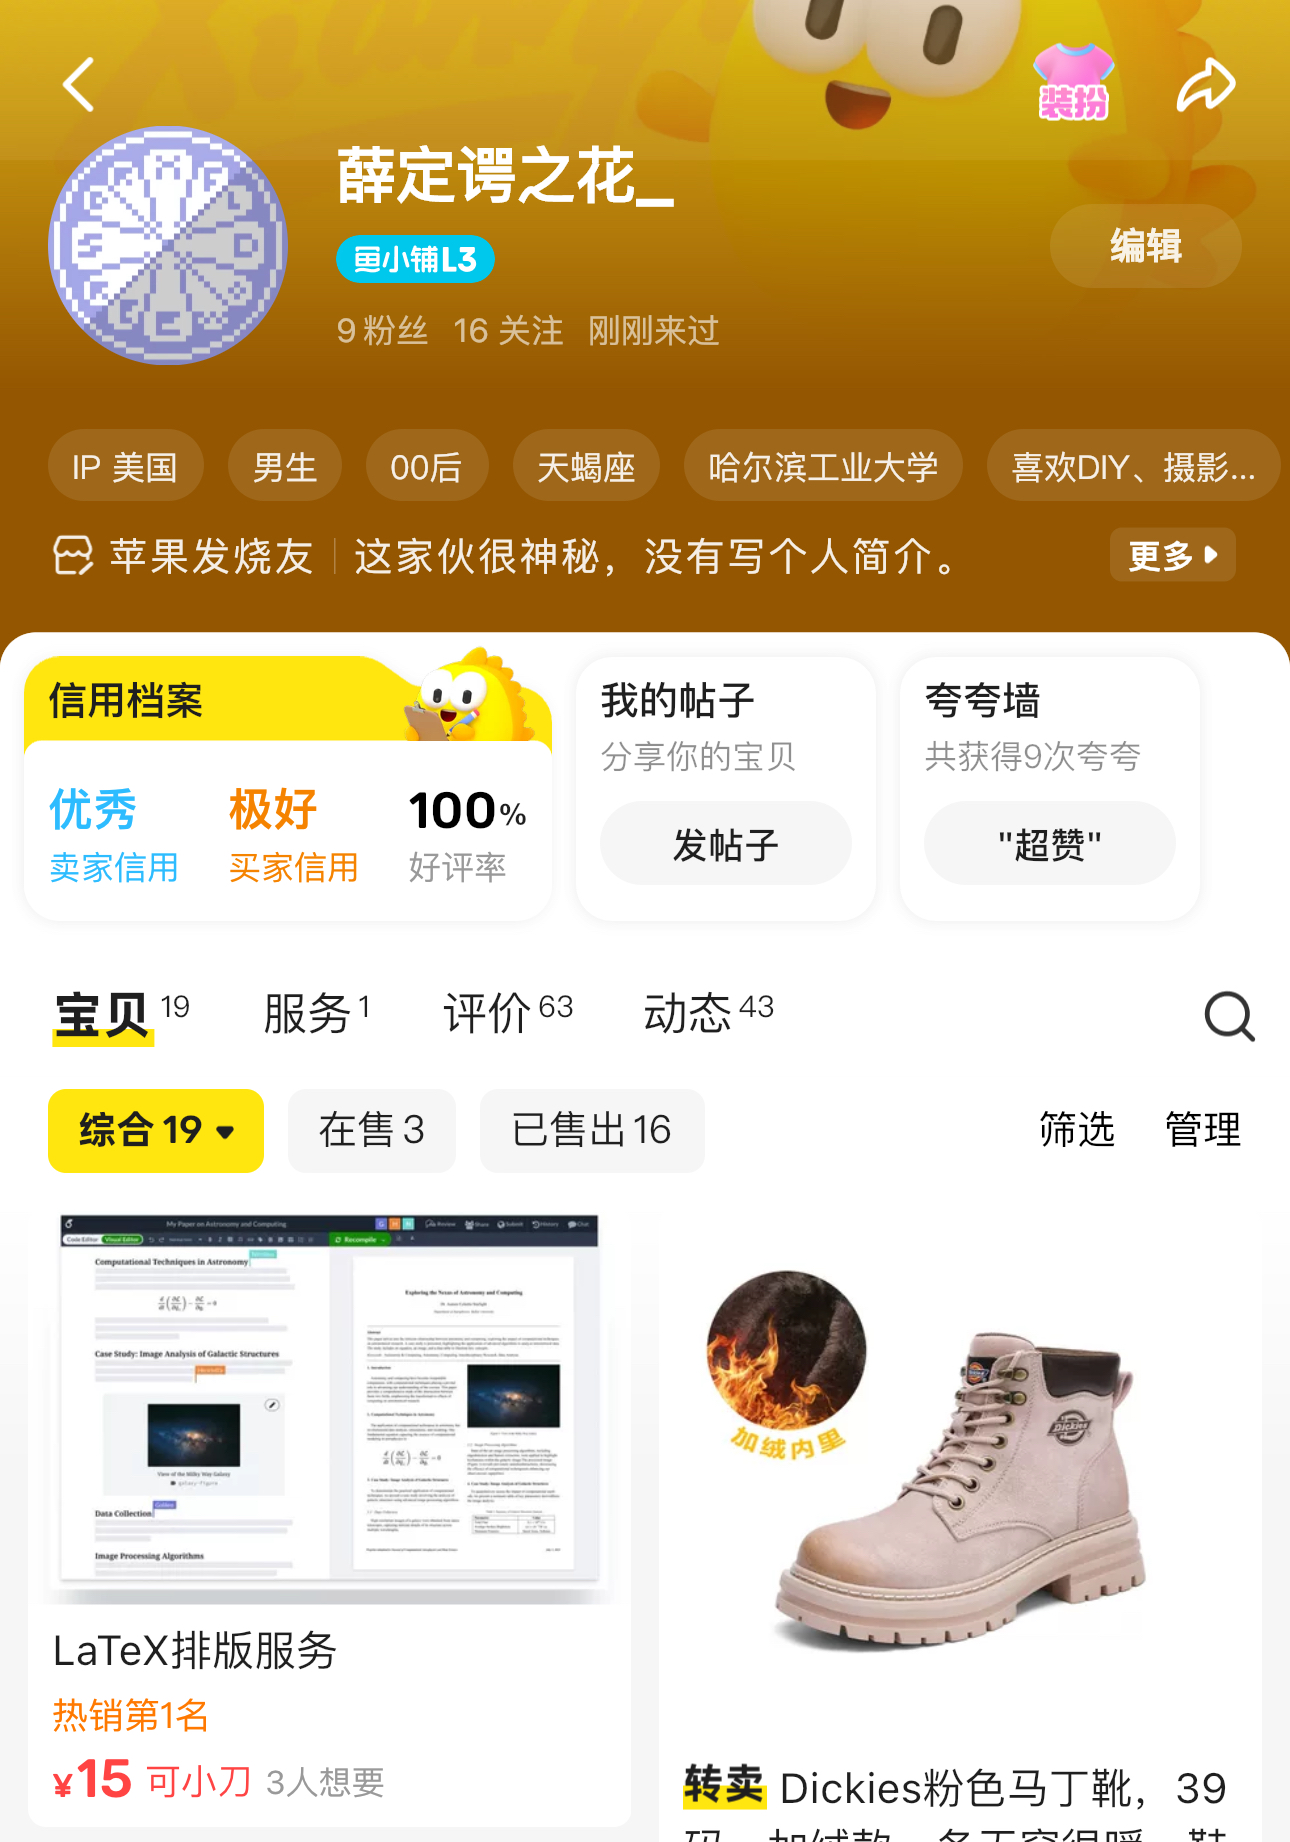
\includegraphics[width=0.3\linewidth]{图/LaTeX排版服务.jpg}
    \bicaption{闲鱼「薛定谔之花\_」\LaTeX 排版服务}{Thank you for your patronage}
    \fignote{如有疑问，欢迎闲鱼联系模板作者或致邮\href{mailto:junhaowu_hit@163.com}{\textcolor{blue}{junhaowu\_hit@163.com}}。}
\end{figure}

图注后的正文文字从此处继续排版，与正文保持一致的行距与缩进格式。

\subsection{续表的使用方法}

跨页表格使用 \verb|longtable| 环境实现，示例如下：

\begin{longtable}{@{}lll@{}}
    \bicaption{表格标题}{Table Title}\\
    \toprule
    列1 & 列2 & 列3 \\
    \midrule
    \endfirsthead
    \bicaption[]{表格标题（续表）}{Table Title (Continued)}\\
    \toprule
    列1 & 列2 & 列3 \\
    \midrule
    \endhead
    \midrule
    \endfoot
    \bottomrule
    \endlastfoot
    数据1 & 数据2 & 数据3 \\
    数据1 & 数据2 & 数据3 \\
    数据1 & 数据2 & 数据3 \\
    数据1 & 数据2 & 数据3 \\
    数据1 & 数据2 & 数据3 \\
    数据1 & 数据2 & 数据3 \\
    数据1 & 数据2 & 数据3 \\
    数据1 & 数据2 & 数据3 \\
    数据1 & 数据2 & 数据3 \\
    数据1 & 数据2 & 数据3 \\
    数据1 & 数据2 & 数据3 \\
    数据1 & 数据2 & 数据3 \\
    数据1 & 数据2 & 数据3 \\
    数据1 & 数据2 & 数据3 \\
    数据1 & 数据2 & 数据3 \\
    数据1 & 数据2 & 数据3 \\
    数据1 & 数据2 & 数据3 \\
    数据1 & 数据2 & 数据3 \\
    数据1 & 数据2 & 数据3 \\
    数据1 & 数据2 & 数据3 \\
    数据1 & 数据2 & 数据3 \\
    数据1 & 数据2 & 数据3 \\
    数据1 & 数据2 & 数据3 \\
    数据1 & 数据2 & 数据3 \\
    数据1 & 数据2 & 数据3 \\
    数据1 & 数据2 & 数据3 \\
    数据1 & 数据2 & 数据3 \\
    数据1 & 数据2 & 数据3 \\
    数据1 & 数据2 & 数据3 \\
    数据1 & 数据2 & 数据3 \\
    数据1 & 数据2 & 数据3 \\
    数据1 & 数据2 & 数据3 \\
    数据1 & 数据2 & 数据3 \\
\end{longtable}
% \input{论文内容/第...章} % 按需添减



% —— 参考文献 —— 毋动
\clearpage
\printbibliography
\addcontentsline{toc}{section}{参考文献}



% —— 附录 ——
\pagebreak
\begin{appendices}
    \resetappendixcounters
    \section{索引的使用方法}

使用 \verb|\index{}| 命令添加索引标记，格式为"拼音@文字"，拼音用于确定排序。

索引标记的基本原则是：标注\textbf{读者可能需要快速定位的内容}。具体建议如下：

\subsection{适合标注的内容}

\begin{itemize}
    \item \textbf{专业术语与核心概念}：在首次定义或解释处必须标注，后续重要论述处可酌情标注。例如：量子纠缠\index{liangzijiuchan@量子纠缠}是指……
    \item \textbf{重要人名与机构名}：例如：广西大学\index{guangxidaxue@广西大学}于……
    \item \textbf{物理量符号}：在首次出现定义处标注。例如：热扩散系数 $\alpha$\index{rekuosanxishu@热扩散系数}表示……
    \item \textbf{方法与模型名称}：例如：最小二乘法\index{zuixiaoerchengfa@最小二乘法}……
\end{itemize}

\subsection{不适合标注的内容}

\begin{itemize}
    \item 目录、摘要、参考文献中的词条
    \item 同一页中重复出现的词条（每页仅标注一次）
    \item 过于通用的词汇（如"研究""方法""结果"等）
    \item 图表题注中的词条
\end{itemize}

需要说明的是，学位论文通常不要求编制索引。若不需要此功能，注释或删除 \verb|\clearpage\gxuprintindex| 即可。
    \clearpage
\section{第二个附录}

附录内容……
  % \input{论文内容/附录...} % 按需添减
\end{appendices}



% —— 索引 —— 不需要则注释/删掉
\clearpage
\gxuprintindex



% —— 成果 ——
\clearpage
\section*{攻读学位期间取得成果情况}
\addcontentsline{toc}{section}{攻读学位期间取得成果情况}
\noindent 发表论文：

\begin{enumerate}[shuzi]
    \item 《Engineering Applications of Artificial Intelligence》期刊发表论文2篇，SCI一区TOP 期刊, 第一作者。
    \item 在《Journal of Cleaner Production》期刊发表论文1篇， SCI一区 TOP 期刊, 第二作者。
\end{enumerate}

\noindent 软著:

\begin{enumerate}[shuzi]
    \item 于2022年04月在中国国家版权局获得4项软著
    \item 于2022年06月在中国国家版权局获得1项软著
\end{enumerate}



% —— 致谢 ——
\clearpage
\section*{致谢}
\addcontentsline{toc}{section}{致谢}
\fangsong % 致谢用仿宋字体，注释/删掉则使用宋体
\input{论文内容/致谢}
\end{document}